\chapter{アプリケーションのアイディア}

\section{コンセプト}
BuLoはバスに乗り遅れたくないひとのためのバスロケーションアプリである.従来のバスロケーションアプリやGoogle Mapsなどの地図アプリとは異なり,バスの位置や遅延情報をリアルタイムにわかりやすく把握することができる.また,“ひとめぼれ”するバスロケーションアプリをめざしている.本グループは”ひとめぼれ”を以下の2つと考える.まず1つ目にアプリのデザインに対する”ひとめぼれ”である.これはアプリを使うきっかけとなるものである.2つ目にアプリ全体を通しての体験への”ひとめぼれ”である.これは,アプリを使い続けるきっかけになると考える.
\bunseki{大津武琉}

\section{機能}
\subsection{住所を登録}
このアプリの対象ユーザは通勤・通学にバスを利用する人であるため,自宅と職場の住所を登録する機能を搭載する.対象ユーザの使用するルートは変わらないため,最初に登録することで,2回目以降は検索をする手間を省いている.

\begin{figure}[htbp]
    \centering
    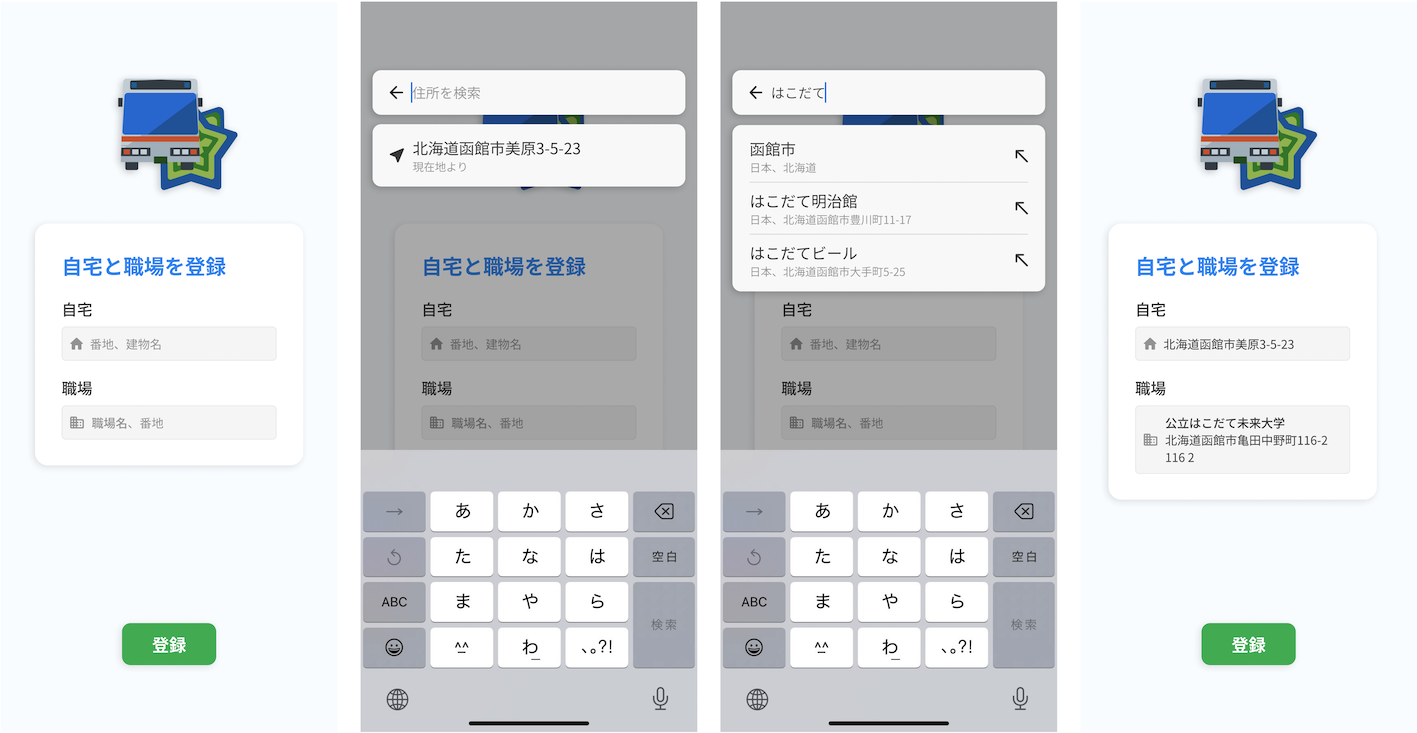
\includegraphics[width=12cm]{images/feature_registration.png}
    \caption{住所登録機能}
    \label{fig:feature_registration}
\end{figure}

\subsection{Time-Distance View}
これは人とバス,バス停の距離を時間的グラフに表すことでパッとみてユーザとバスの位置関係を把握することができる.実装方法は以下の図に示す.

\begin{figure}[htbp]
    \centering
    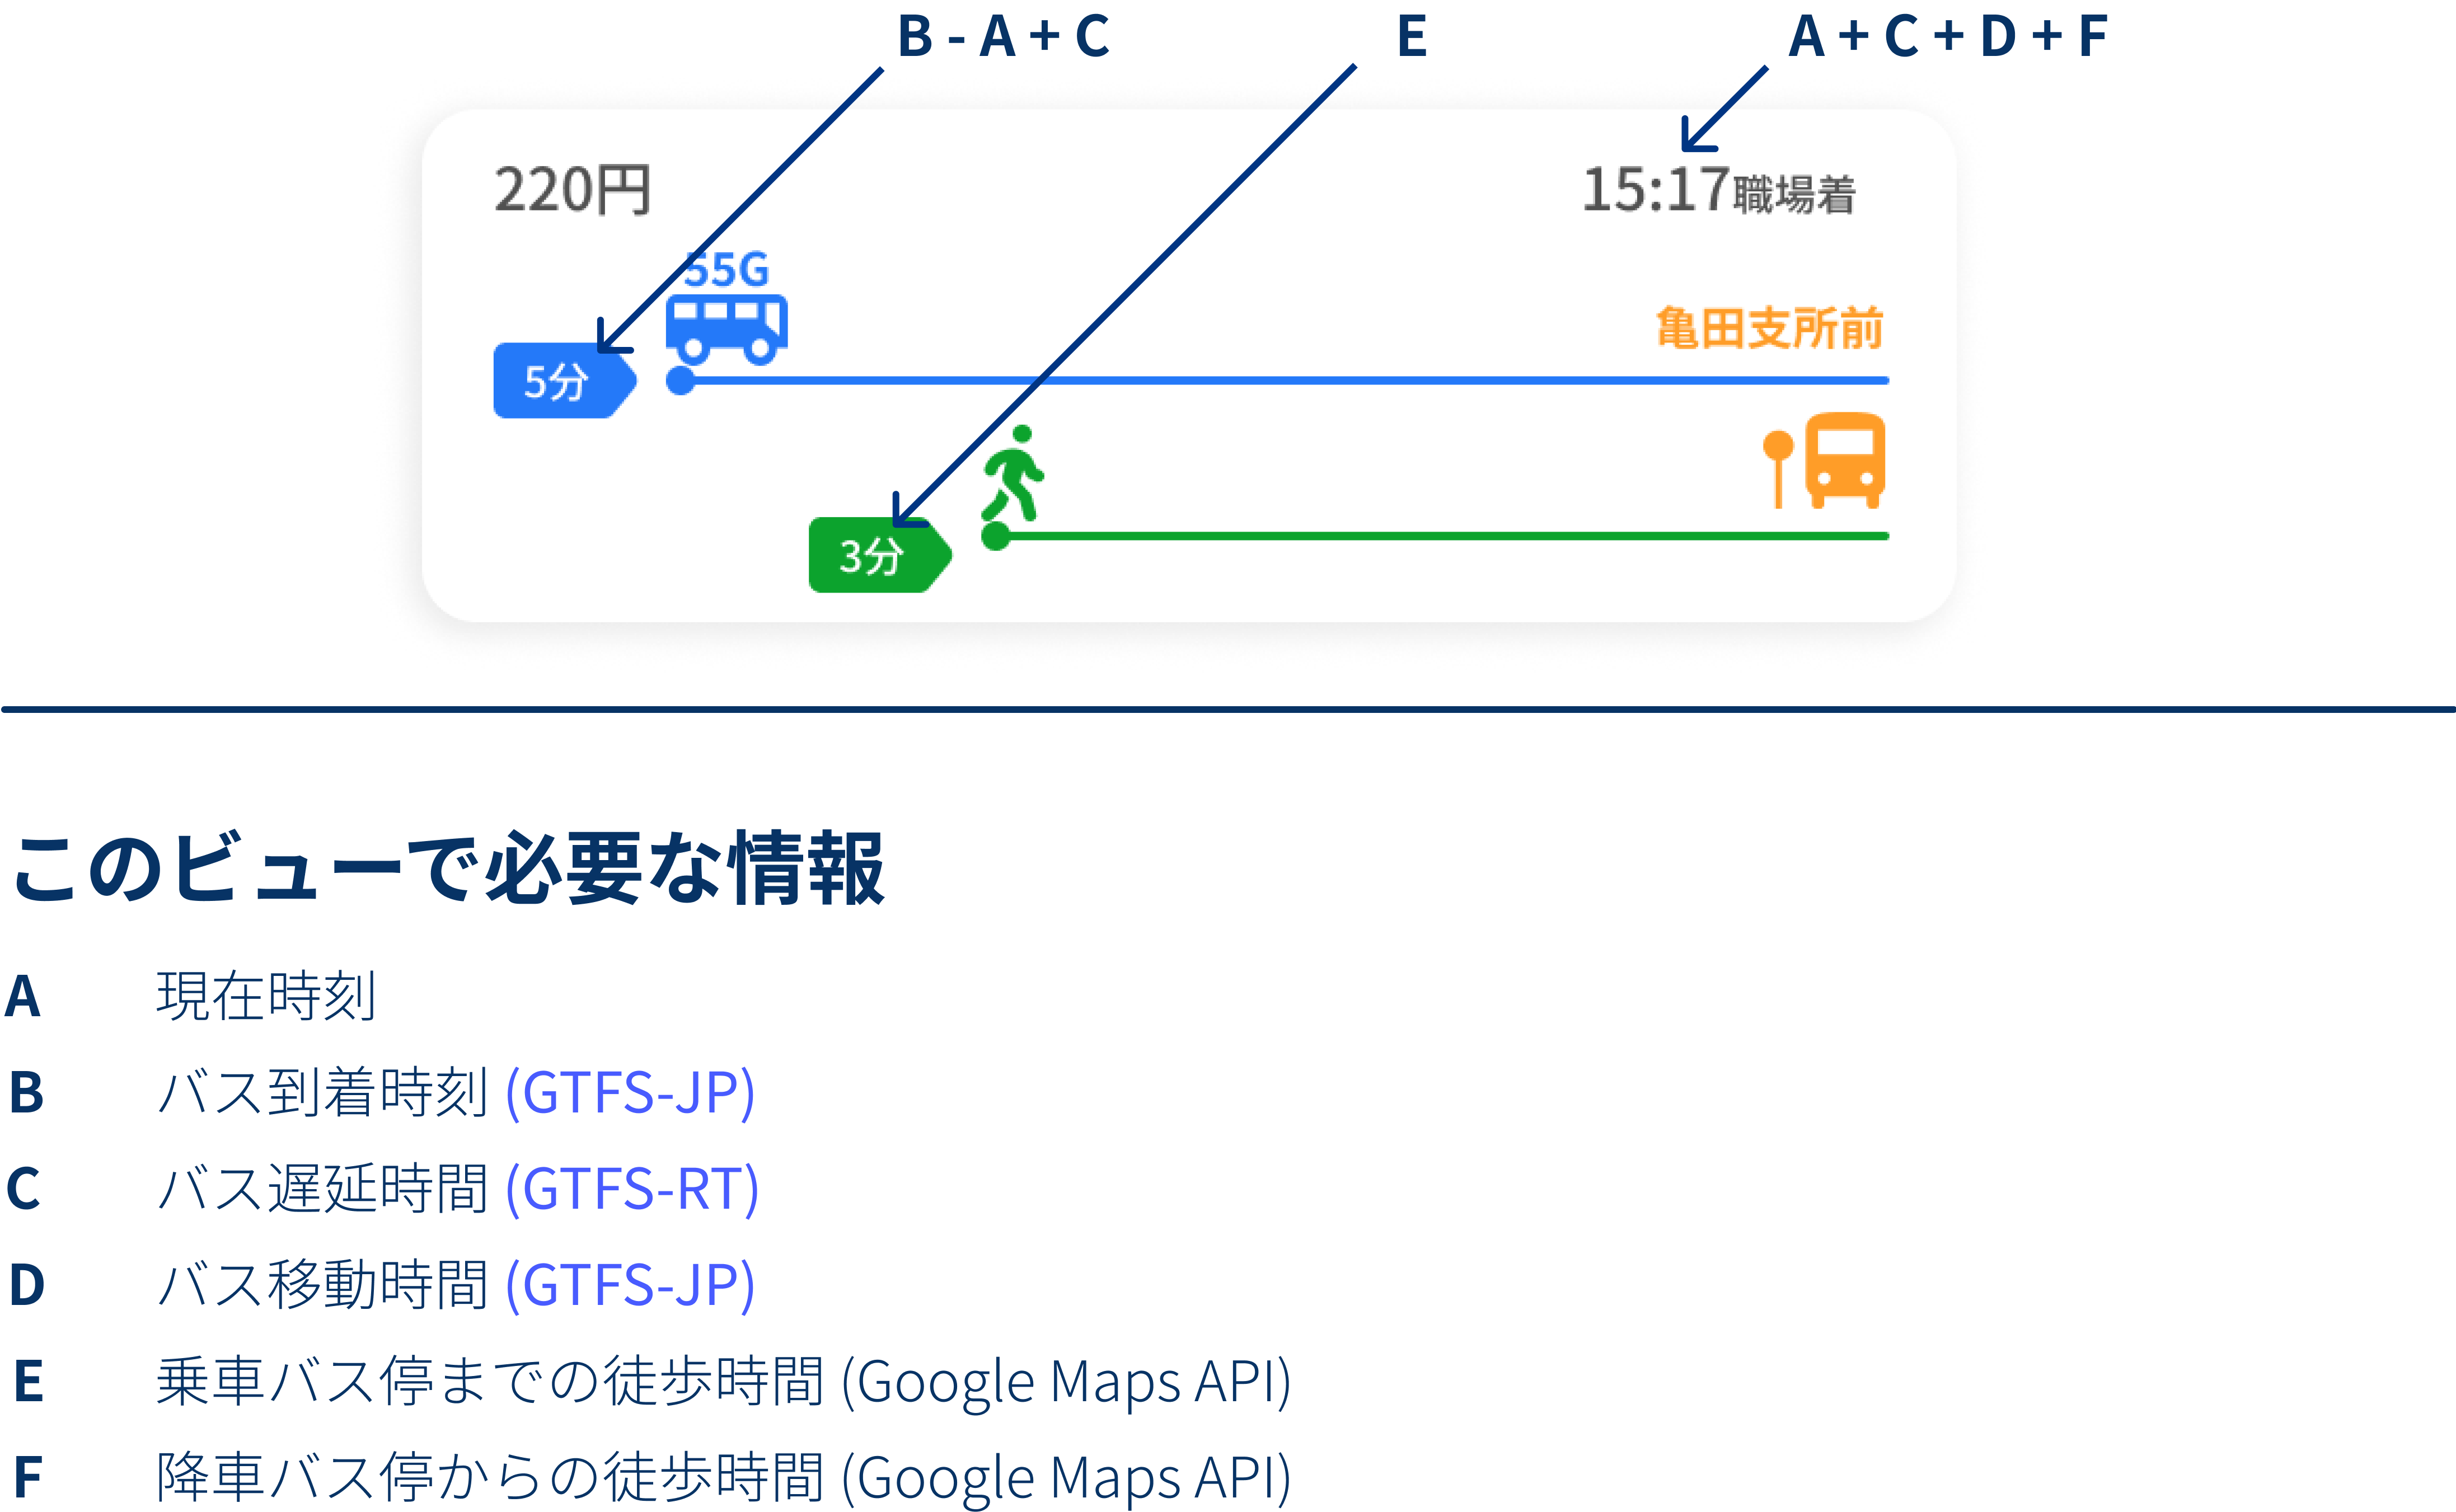
\includegraphics[width=12cm]{images/feature_timedistanceview.png}
    \caption{Time-Distance View}
    \label{fig:feature_timedistanceview}
\end{figure}

\subsection{バスの位置情報}
地図上でバスとユーザの位置を確認することができる.

\begin{figure}[htbp]
    \centering
    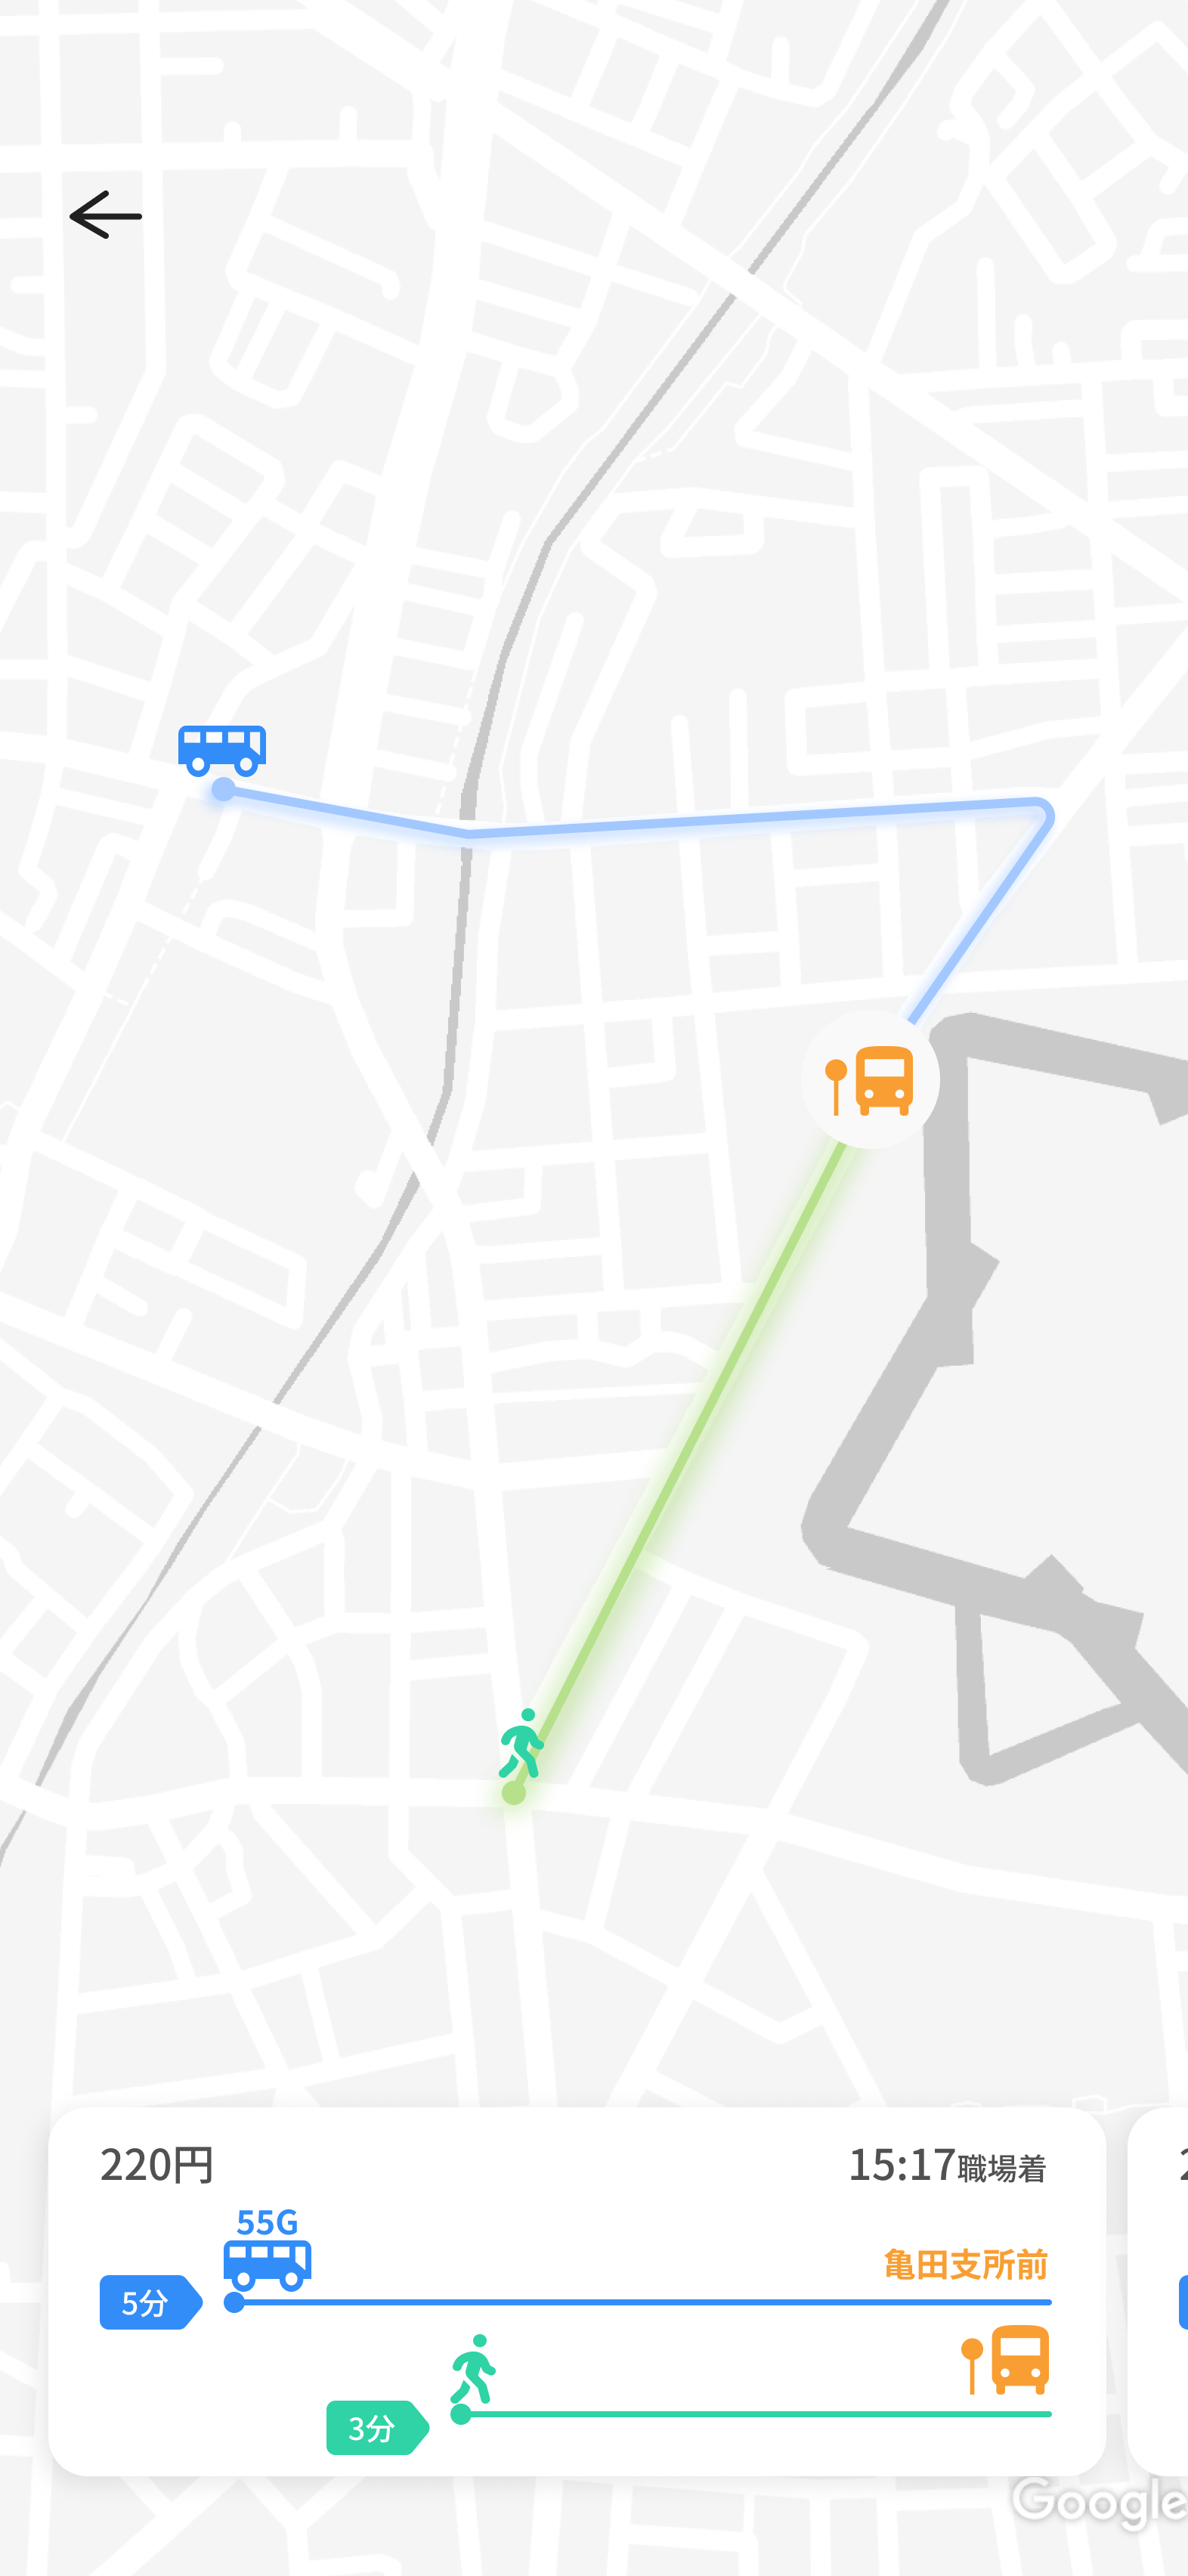
\includegraphics[width=4cm]{images/feature_routeview.png}
    \caption{バス位置情報閲覧機能}
    \label{fig:feature_routeview}
\end{figure}
\bunseki{大津武琉}
